\documentclass[a4paper, handout]{beamer}
\usepackage{graphicx}
\graphicspath{ {./images/} }

\begin{document}

\begin{frame}
	\frametitle{Overleven}
	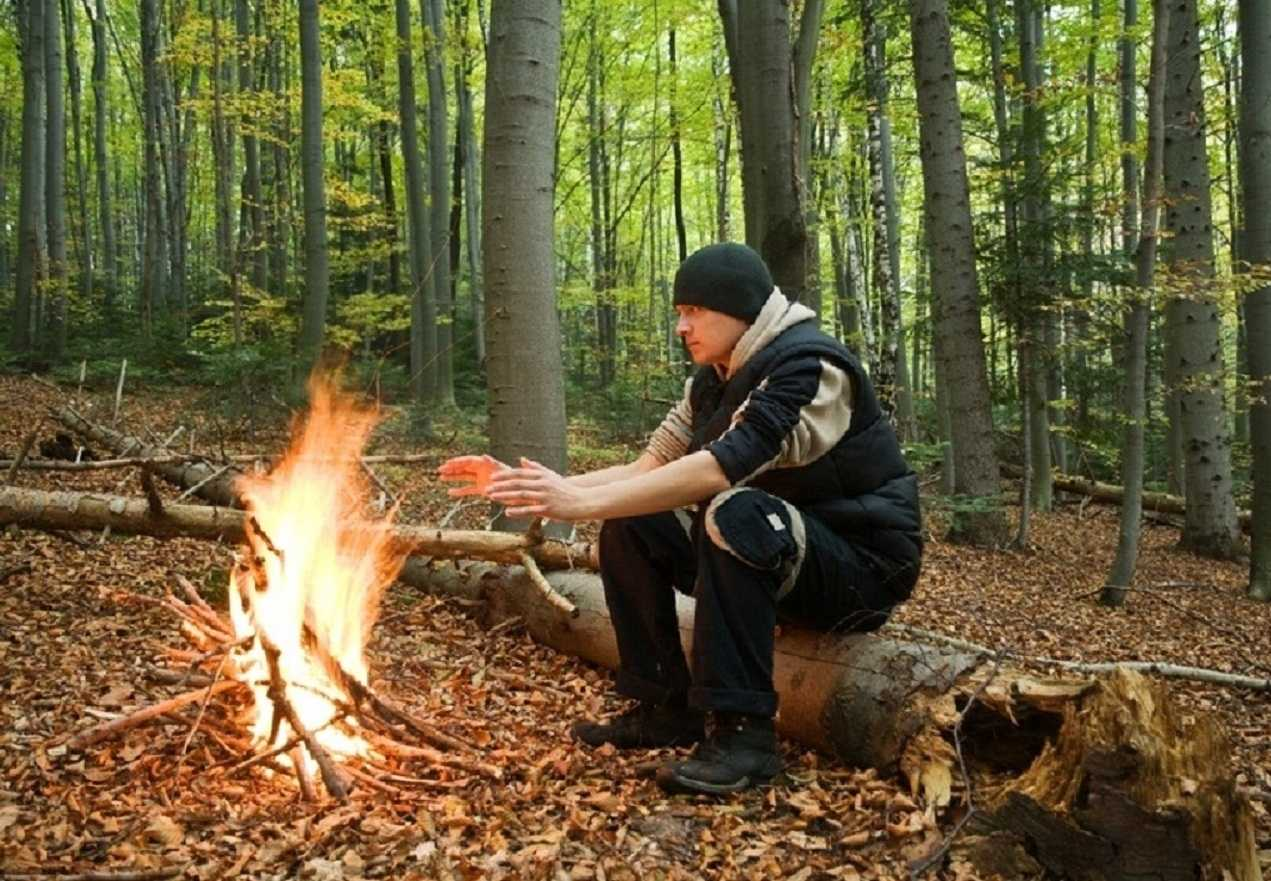
\includegraphics[width=\linewidth]{man-bij-vuur}
\end{frame}
\begin{frame}
	\frametitle{Hoe te overleven}
	Om te kunnen overleven heb je nodig:
	\begin{enumerate}
		\item{Water}
		\item{Voedsel}
		\item{Beschutting}
		\item{Vuur}
	\end{enumerate}
\end{frame}

\begin{frame}
	\frametitle{Vuur is belangrijk}
	\begin{enumerate}
		\item{Om water te zuiveren}
		\item{Warmte}
		\item{Om te koken}
		\item{Bescherming tegen wilde dieren}
	\end{enumerate}
\end{frame}

\begin{frame}
	\frametitle{Vuur basis}
	Vuur krijg je alleen maar als de volgende dingen er zijn:
	\begin{enumerate}
		\item{Brandstof}
		\item{Zuurstof}
		\item{Hitte}
	\end{enumerate}
	Wij gaan verder kijken naar wrijvingsvuur.
\end{frame}

\begin{frame}
	\frametitle{Wrijvingsvuur}
	Wij gebruiken als basis	
	\begin{description}
		\item[Brandstof] pluizen, stro, twijgjes en groter hout
		\item[Zuurstof] 20 procent van de lucht is zuurstof
		\item[Hitte] wrijving!
	\end{description}
\end{frame}

\begin{frame}
	\frametitle{Vuurboog}
	Voor een vuurboog heb je nodig:
	
	\begin{description}
		\item[Snaar] stevig stuk touw van minimaal een meter
		\item[Boog] kromme stok van 50 tot 70 centimeter lang
		\item[Dop] een stuk steen met een holte om druk te leveren
		\item[Opvanger] stukje dun hout om het kooltje te vangen
		\item[Boor] een rechte tak van 15 tot 20 millimeter dik en tussen de 15 en 30 centimeter lang
		\item[Vuurbord] een plankje van 15 tot 25 millimeter dik, minimaal twee keer de breedte van de dikte van de boor. En 20 centimeter lang.
	\end{description}
\end{frame}

\begin{frame}
	\frametitle{Houtsoorten}
	Voor een vuurbord en boor gebruik je het liefst dezelfde soort hout.

	De beste soorten zijn zachte houtsoorten zoals:
	\begin{enumerate}
		\item{Naaldbomen}
		\item{Wilg}
		\item{Populier}
	\end{enumerate}
	
\end{frame}

\begin{frame}
	\frametitle{Boor maken}
	Een vuurboor is een potlood met gum in het groot en op zijn kop. Met de botte kant gaan we boren in het vuurbord, want we willen veel wrijving.

	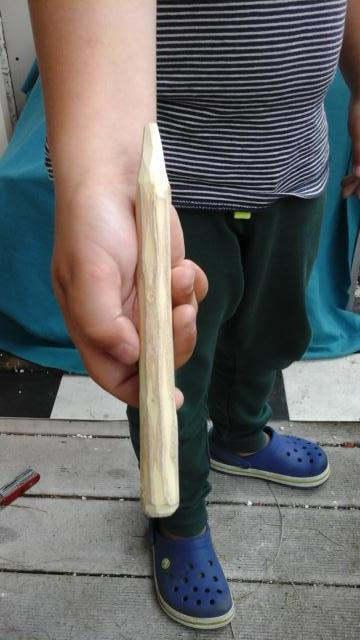
\includegraphics[scale=1.2]{vuurboor}
\end{frame}

\begin{frame}
	\frametitle{Vuurboog maken}
	Je kunt aan de uiteindes van de boog een gleufje zagen waarin je de snaar bevestigt.

	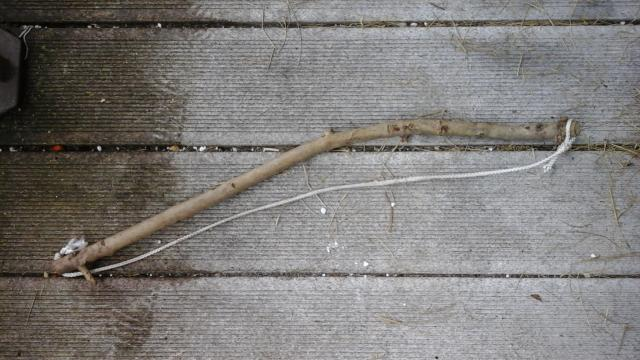
\includegraphics[scale=0.4]{vuurboog}

\end{frame}
\begin{frame}
	\frametitle{Aan de slag}
	\begin{enumerate}
		\item{Vogelnestje maken}
		\item{Indraaien op het vuurbord}
		\item{Inkeping voor het stof maken}
		\item{Boren voor een kooltje}
		\item{Kooltje in het vogelnestje doen en aanblazen}
	\end{enumerate}

	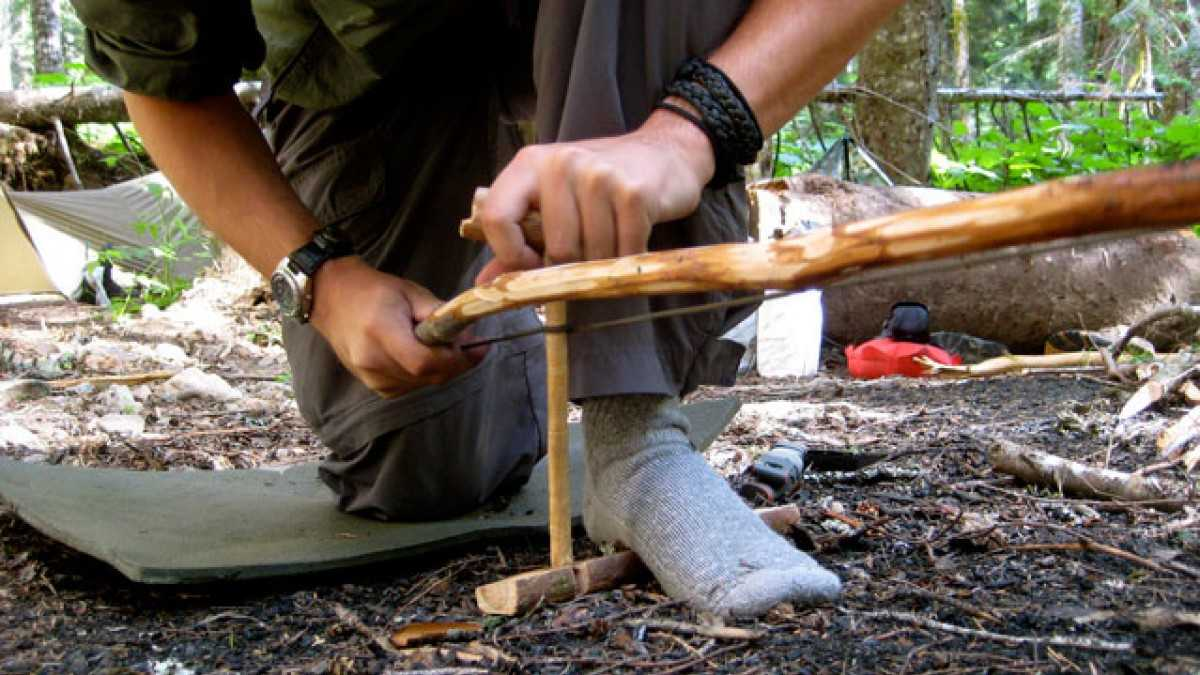
\includegraphics[width=\linewidth]{vuurboog-actie}

\end{frame}
\end{document}

